% !Mode:: "TeX:UTF-8"
% !TEX program  = xelatex

\documentclass{cumcmthesis}
%\documentclass[withoutpreface,bwprint]{cumcmthesis} %去掉封面与编号页,电子版提交的时候使用。
\usepackage{tikz}
\usetikzlibrary{positioning, shapes.geometric}
\usetikzlibrary{calc}

\tikzstyle{format}=[rectangle,draw,thin,fill=white]  
%定义语句块的颜色,形状和边
\tikzstyle{test}=[diamond,aspect=2,draw,thin]  
%定义条件块的形状,颜色
\tikzstyle{point}=[coordinate,on grid,]  
\tikzstyle{startstop} = [rectangle, rounded corners,minimum height=0.7cm,text centered, draw=black]
\tikzstyle{io} = [trapezium, trapezium left angle=70, trapezium right angle=110,  minimum height=0.7cm, text centered, draw=black]
\tikzstyle{process} = [rectangle,  minimum height=0.7cm, text centered, draw=black]
\tikzstyle{decision} = [diamond, minimum height=0.7cm, text centered, draw=black]
\tikzstyle{arrow} = [thick,->,>=stealth]
\tikzstyle{every node}=[font=\normalsize, node distance = 13mm]
\usepackage{pdfpages}
\usepackage[framemethod=TikZ]{mdframed}
\usepackage{url}   % 网页链接
\usepackage{subcaption} % 子标题

\usepackage{fancyhdr}
\title{高比例风电电力系统储能运行及配置分析}


\begin{document}
% \maketitlen
	\setcounter{page}{2}
 \begin{abstract}
 	本文围绕可再生能源输出功率强随机波动性导致系统运行中功率实时平衡困难以及储能成本相对昂贵,利用储能平衡系统功率将增加系统运行成本等问题,通过计算得到的结果分析风电装机替代火电机组造成的影响,并建立优化模型来解决供电平衡问题。
 	
 	针对问题一:输入一天的负荷曲线利用等微增率法建立优化模型求出三台机组的最优发电计划,经过判断筛选得到正确的发电计划;随后将其代入题目所给公式求得煤使用量,即可得到火电运行成本;随后求出碳捕集成本;最后将火电运行成本与碳捕集成本相加求出火电成本,即可求出单位供电成本。
 	
 	针对问题二:首先求出风电机组替换机组3后的净负荷曲线,根据净负荷曲线并采用等微增率法求出机组1和2的发电计划,经过判断筛选得到正确的发电计划,根据发电计划算出弃风功率曲线,并对弃风功率进行积分即可求出总的弃风量;最后根据出机组总功率与负荷功率之差的最小值计算出风机功率的富余量。
 	
 	针对问题三:首先求出风电机组替换机组2后的净负荷曲线,根据净负荷曲线并采用等微增率法求出机组1和2的发电计划,经过判断筛选得到正确的发电计划;随后算出弃风功率曲线与失负荷功率曲线,求积分可得总的弃风量以及总失负荷量;最后根据机组总功率与负荷功率之差的最小值计算出风机功率的缺额量。
 	
 	针对问题四:根据问题二和问题三,可以得到弃风总量,从而计算出弃风损失;接着计算出失负荷功率并对其求积分得到失负荷量(问题二中不需要考虑失负荷量),并计算出失负荷损失,并如问题一所述求得火电成本,从而求出发电总成本,即可得到系统单位供电。
 	
 	针对问题五:首先求出风电机组替换机组2,3后的净负荷曲线,根据净负荷曲线并采用等微增率法求出机组1的发电计划;并算出总的弃风量以及总失负荷量,接着算出失负荷损失、火电成本和风电运维成本;接着结合计算出的投资成本和运维成本即可求得储能成本,最后求出发电总成本即可求得单位供电成本。
 	
 	针对问题六:由求解上述问题所得到风电装机300MW替代机组3、风电装机600MW替代机组2时所得的功率平衡图以及相关指标统计分析出风电替代容量的递增会破坏系统的功率平衡,对系统的供电能力带来了不稳定性与波动性。但同时系统单位供电成本会随着风电替代容量的递增而减少。
 	
 	针对问题七:我们针对装机容量1200MW替代机组2,3的情况分析功率平衡所存在的问题,通过建立以最优供电成本为目标、储能功率和储能容量为决策变量的优化模型,并采用遗传算法计算上述模型,得到该系统最优供电成本的功率平衡解决方案。


\keywords{等微增率;弃风量;最优功率;失负荷量}
\end{abstract}
\pagestyle{plain}
\fancyfoot[C]{\thepage}

  \section{无风电接入时系统单位供电成本}
  \subsection{本题解题流程}\label{l}
  \begin{figure}[H]
  	\centering
  	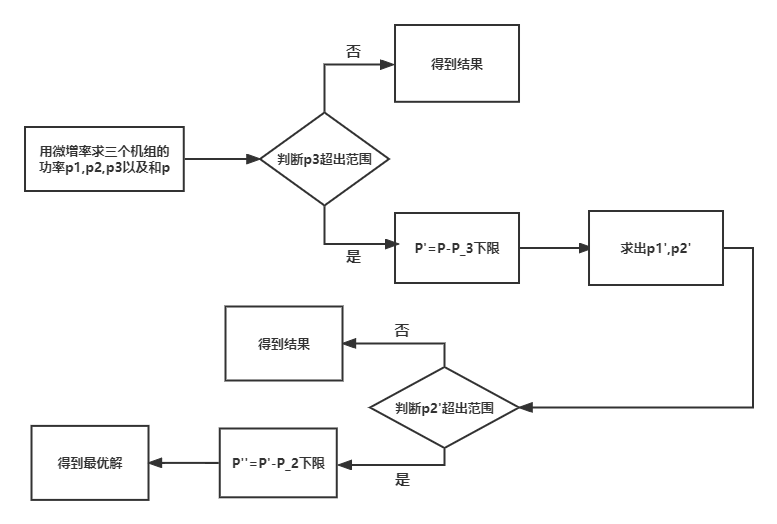
\includegraphics[width=1\textwidth]{f2}
  	\caption{第一题最优功率求解过程}
  	\label{fig:circuit-diagram}
  \end{figure}
  
  上图是第一题最优功率求解流程图,其过程如下:
  
  \begin{enumerate}
  	\item 三机组求解最优功率
  	\item 判断三机组功率是否超出范围
  	\item 若超出范围,则判断是第几号机组超限,将其剔除再使用其他二者进行双机组最优功率求解
  	\item 判断所得双机组最优功率解是否在范围内
  	\item 若超出范围,则未超限机组功率为剩余目标功率与超限机组功率限制之差
  \end{enumerate}
  \subsection{数据处理}\label{数据处理}
  附件一中使用的数据是标幺值($ p.u. $),因此需要将其转换为真实值。其转换公式如下:
  
  \begin{equation}\label{key}
  		A=a\times A_{B}
  \end{equation}
  
  式中:A为数据的真实值,a为标幺值($ p.u. $),$ A_{B} $为数据的基准值。
  
  将附件一中的负荷、风电功率数据处理,存放于同一表(\textbf{附件一.xlsx})中。其中:\textbf{l900}为负荷的真实功率,\textbf{w300}为装机容量为300MW时的风机功率,\textbf{w600}为装机容量为600MW时的风机功率,\textbf{w900}为装机容量为900MW时的风机功率。
  
  数据处理部分后文不再赘述。
  \subsection{三机组等微增率最优解}\label{equalIR3}
  三机组等微增率最优解共需要计算3个参数,即机组1最优功率$ P_{1} $、机组2最优功率$ P_{2} $、机组3最优功率$ P_{3} $,其需要传入的参数为:目标功率$ P_{d} $和各机组煤耗量系数$ a\texttt{,}b\texttt{,}c $。
  
  根据式\ref{target},写出三台机组的目标函数如下:
  
  \begin{equation}\label{key}
  	\left\{\begin{matrix}
  		c_{1}&=0.226 p_{1}^{2} + 30.42 p_{1} + 786.8\\
  		c_{2}&=0.588 p_{2}^{2} + 65.12 p_{2} + 451.32\\
  		c_{3}&=0.785 p_{3}^{2} + 139.6 p_{3} + 1049.5
  	\end{matrix}\right.
  \end{equation}
  
  分别在上述目标函数对$ p_{i} $求偏导,可得:
  \begin{equation}\label{key}
  	\left\{\begin{matrix}
  		\dfrac{\partial c_{1}}{\partial p_{1}}&=0.452 p_{1} + 30.42\\
  		\dfrac{\partial c_{2}}{\partial p_{2}}&=1.176 p_{2} + 65.12\\
  		\dfrac{\partial c_{3}}{\partial p_{3}}&=1.57 p_{3} + 139.6
  	\end{matrix}\right.
  \end{equation}
  
  由约束条件可知:
  
  \begin{equation}\label{key}
  	\sum_{i=1}^{3}p_{i}=p_{d}
  \end{equation}
  
  且:
  
  \begin{equation}\label{key}
  	\dfrac{\partial c_{1}}{\partial p_{1}}=\dfrac{\partial c_{2}}{\partial p_{2}}=\dfrac{\partial c_{3}}{\partial p_{3}}
  \end{equation}
  将上述方程求解即可得到单次三机组等微增率最优解。
  
  \subsection{双机组等微增率最优解}\label{sjzdwzl}
  双机组等微增率最优解算法与三机组类似,其目标函数与偏导函数为2个,共计2条方程。通过约束条件与偏导函数即可求解双机组等微增率最优解。
  
  \subsection{算法代码实现}
  将\ref{equalIR3}中的过程可以用如下流程图表示:
  
  \begin{figure}[H]  
  	\centering
  	
  	\scriptsize  
  	
  	%像素点,用于连接转移线
  	\begin{tikzpicture}[node distance=2cm]
  		%定义流程图具体形状
  		\node (start1) [startstop] {传入目标函数};
  		\node (in1) [process, below of=start1] {计算目标函数的对$ p_{i} $的偏导数};
  		\node (pro1) [process, below of=in1,] {建立约束条件};
  		\node (pro2) [process, below of=pro1] {通过偏导是方程组和约束条件建立方程组};
  		\node (stop1) [startstop, below of=pro2]{求解};
  		
  		%连接具体形状
  		\draw [arrow](start1) -- (in1);
  		\draw [arrow](in1) --  (pro1);
  		\draw [arrow](pro1) -- (pro2);
  		\draw [arrow](pro2) --  (stop1);
  	\end{tikzpicture}
  	\caption{三机组等微增率计算流程}
  	\label{dthz}
  \end{figure} 
  
  
  
  
  
  \subsection{本题求解过程}

 
  \subsubsection{煤使用量及运行维护成本计算}\label{ll}
  煤使用量$ F $计算公式如下:
  \begin{equation}\label{coalUsc}
  	F_{i}=a_{i}P_{i}^{2}+b_{i}P_{i}+c_{i}
  \end{equation}
  
  其中$ a\texttt{,}b\texttt{,}c $为各机组煤耗量系数。
  
  
  \subsubsection{碳捕集成本}\label{lll}
  当日发电量为发电功率在时间上的积分,因此可以根据发电计划对时间积分即可求出当日发电量。碳捕集量为$ \texttt{当日发电量}\times \texttt{机组碳排放量参数} $。
  
  \subsubsection{单位供电成本}
  系统总负荷量为系统负荷功率在时间上的积分,因此可以根据系统负荷曲线进行系统总负荷量的求解。
  
  根据定义,单位供电成本为$ \texttt{系统总成本}/\texttt{系统总负荷量} $,而系统总成本为$ \texttt{火电成本+}$  $\texttt{风电成本+储能成本+弃风损失+失负荷损失} $,本题中,后四者均无需考虑,因此在本题中系统总成本为$ \texttt{火电成本} $,即$ \texttt{火电运行成本+碳捕集成本} $。
  
  
  \subsection{求解结果}
  
  \subsubsection{发电计划曲线}
  % TODO: \usepackage{graphicx} required
  \begin{figure}[H]
  	\centering
  	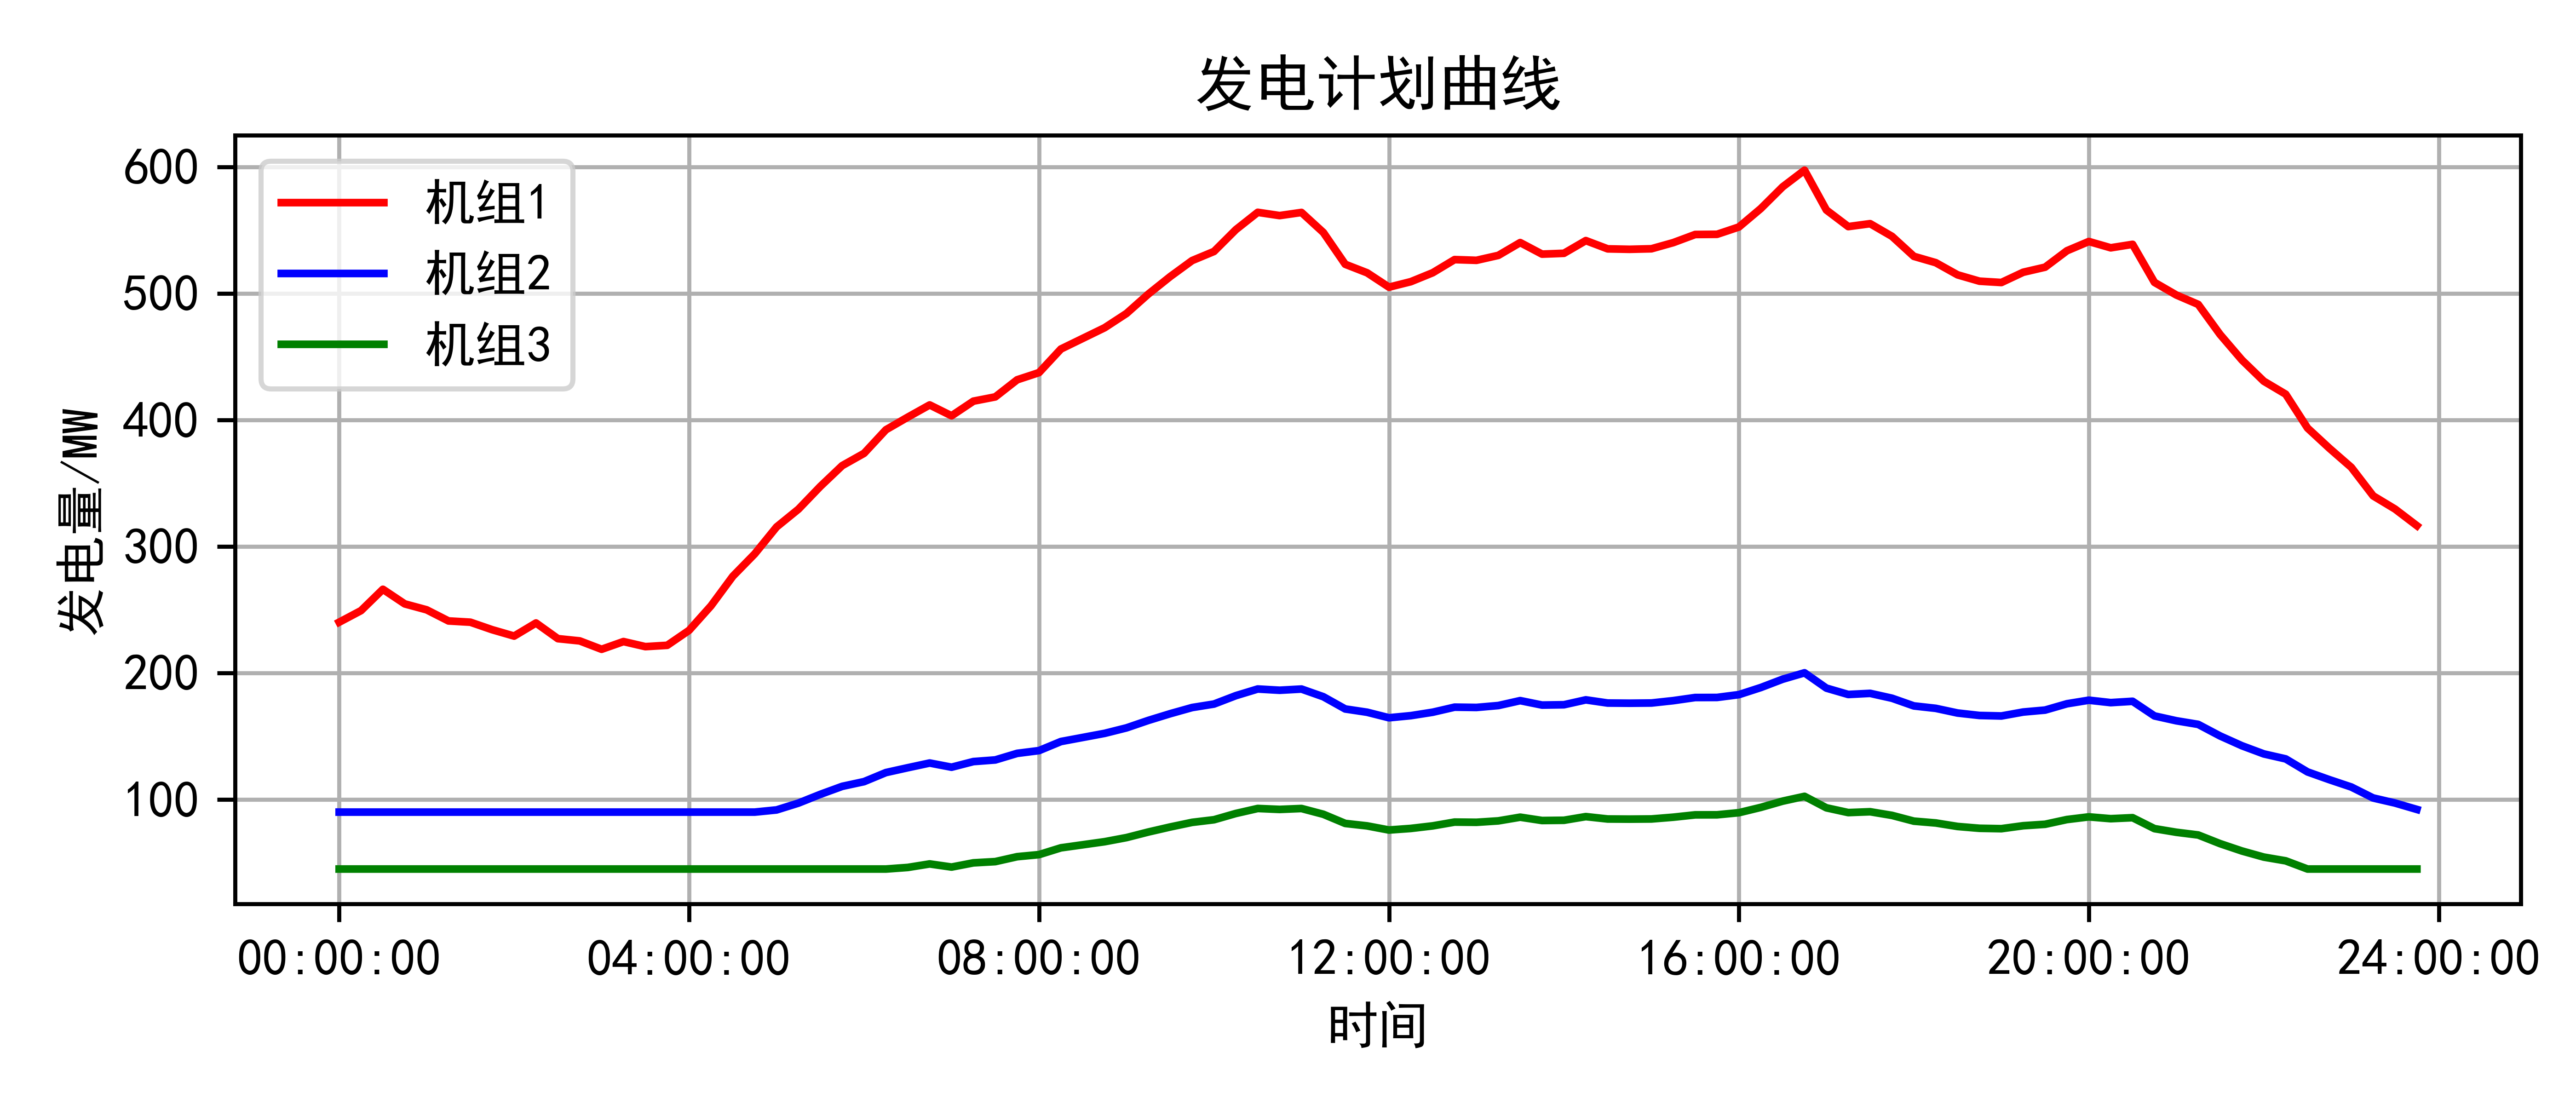
\includegraphics[width=1\linewidth]{figures/三台火电机组最优发电曲线}
  	\caption{机组1、2、3发电计划曲线}
  	\label{fig:screenshot001}
  \end{figure}
  
  \subsubsection{风电电量占比为0时系统相关指标统计}
  \begin{table}[H]
  	\centering
  	\caption{风电电量占比为0时系统相关指标统计}
  	\label{tab:my-table}
  	\begin{tabular}{lllll}
  		\toprule[1.5pt]
  		\begin{tabular}[c]{@{}l@{}}碳捕集成本\\ (元/t)\end{tabular} &
  		\begin{tabular}[c]{@{}l@{}}火电运行成本\\ (万元)\end{tabular} &
  		\begin{tabular}[c]{@{}l@{}}碳捕集成本\\ (万元)\end{tabular} &
  		\begin{tabular}[c]{@{}l@{}}总发电成本\\ (万元)\end{tabular} &
  		\begin{tabular}[c]{@{}l@{}}单位供电成本\\ (元/KWh)\end{tabular} \\ 
  		\midrule[1pt]
  		0   & 244.573 & 0       & 244.573 & 0.158 \\
  		60  & 244.573 & 68.288  & 312.861 & 0.202 \\
  		80  & 244.573 & 91.05   & 335.624 & 0.216 \\
  		100 & 244.573 & 113.813 & 358.386 & 0.231 \\ 
  		\bottomrule[1.5pt]
  	\end{tabular}
  \end{table}

  \subsection{代码封装及实现}
 将节\ref{equalIR3}中的过程封装为函数\textbf{equalIR\_algorithm\_3},其详细代码见\textbf{附录B-Python程序源代码-第一题-第一题:等微增率求解发电曲线.py}。其中传入参数为$ P_{d} $,即目标功率;返回结果为三个机组的最优功率值$ P_{1}\texttt{,}P_{2}\texttt{,}P_{3} $。
 
 双机组等微增率求解封装为函数\textbf{equalIR\_algorithm\_2},其详细代码见\textbf{附录B-Python程序源代码-第一题-第一题:等微增率求解发电曲线.py}。其中传入参数为$ P_{d} $,即目标功率;返回结果为两个机组的最优功率值$ P_{1}\texttt{,}P_{2}$。
 
 节\ref{l}中最优功率求解过程范围是否超限使用函数\textbf{judge}判断,其传入参数为p\texttt{:功率,}up\texttt{:功率上限,}down\texttt{:功率下限},其详细代码见\textbf{附录B-Python程序源代码-第一题-第一题:等微增率求解发电曲线.py}。
 
 将将节\ref{ll}各机组煤耗量系数封装为函数\textbf{fireStationCoalCost},将运行维护成本(0.5倍的煤耗成本)封装为\textbf{fireStationRunCost},上述函数存放在\textbf{附录B-Python程序源代码-第一题-fireStationCost.py}中。
 
 将节\ref{lll}的计算过程封装为函数\textbf{carbonEmission},其传入参数为:1、发电计划,2、机组碳排放量参数;返回结果为碳捕集量。碳捕集成本为$ \texttt{碳捕集量}\times \texttt{碳捕集单价} $。据此即可计算碳捕集成本。
 
 上述函数存放在\textbf{附录B-Python程序源代码-第一题-fireStationCost.py}中。
 
  
  \newpage
  \section{300MW风机替代机组3后系统功率平衡变化情况分析}
    \subsection{本题求解流程}
    \begin{figure}[H]  
    	\centering
    	
    	\scriptsize  
    	
    	%像素点,用于连接转移线
    	\begin{tikzpicture}[node distance=2cm]
    		%定义流程图具体形状
    		\node (start1) [startstop] {制定火电机组最优发电计划};
    		\node (in1) [process, below of=start1] {计算弃风功率$ P_{wind\ loss} $的曲线};
    		\node (pro1) [process, below of=in1,] {将弃风功率在时间上进行积分,得到弃风量};
    		\node (stop1) [startstop, below of=pro1]{得到结果};
    		
    		%连接具体形状
    		\draw [arrow](start1) -- (in1);
    		\draw [arrow](in1) --  (pro1);
    		\draw [arrow](pro1) --  (stop1);
    	\end{tikzpicture}
    	\caption{第二题求解流程}
    	\label{dthz}
    \end{figure}
	上图是第二题求解的流程图,
	我们先通过等微增率算法计算得出出火电机组1、2的最优发电计划,再计算出弃风功率$ P_{wind\ loss} $的曲线,接着将弃风功率在时间上进行积分,得到弃风量,最后得到结果。

	\subsection{弃风量的计算}\label{qfl}
	弃风功率为系统功率超出负荷所需功率的部分。弃风功率$ P_{wind\ loss} $可以通过下面式子进行表达:
	\begin{equation}\label{qfleq}
		P_{wind\ loss} =P_{fire}+P_{wind}-P_{d}
	\end{equation}
	
	式中:$ P_{fire} $为火电机组功率总和,$ P_{wind} $为风电机组功率。
	
	弃风量为弃风功率在时间上的积分,即:
	\begin{equation}\label{key}
		\texttt{弃风量}=\int_{t_{0}}^{t_{1}}P_{wind\ loss}\mathit{d}t
	\end{equation}
	
	\subsection{失负荷量的计算}\label{sfhl}
	失负荷功率为系统功率小于负荷所需功率的部分。失负荷功率$ P_{load\ loss} $可以通过下面式子进行表达:
	\begin{equation}\label{sfhleq}
		P_{load\ loss} =P_{d}-(P_{fire}+P_{wind})
	\end{equation}
	
	式中:$ P_{fire} $为火电机组功率总和,$ P_{wind} $为风电机组功率。
	
	失负荷量为失负荷功率在时间上的积分,即:
	\begin{equation}\label{key}
		\texttt{失负荷量}=\int_{t_{0}}^{t_{1}}P_{load\ loss}\mathit{d}t
	\end{equation}
	
\subsection{计算弃风量、失负荷量}\label{jsqflsfhl}
将节\ref{qfl}、节\ref{sfhl}中的流程封装为函数\textbf{get\_wind\_loss},其传入参数为:1、风电功率,2、各机组功率,3、负荷功率;返回值为$ \texttt{系统机组总功率之和}-\texttt{负荷功率} $。

对于该函数的返回值可以发现,其正值为起风功率,负值则为失负荷功率。

因此根据弃风量的定义,可以将弃风量封装成函数\textbf{get\_wind\_load},其传入参数为上一函数\textbf{get\_wind\_loss}的返回值,返回值为弃风量。

对于失负荷量,本题中未要求计算,因此在本题代码中未对其进行封装。封装代码在第五题中体现。	

上述函数存放在\textbf{附录B-Python程序源代码-第二题-第二题:弃风.py}中。
\subsection{本题求解过程}

	\subsubsection{火电机组最优功率}
	本题中,风机替代了机组3,根据节\ref{sjzdwzl}中双机组最优功率求解可以计算出机组1、2的最优功率发电曲线。
	
	
	
	\subsubsection{计算风机功率富余量}
	通过节\ref{jsqflsfhl}中的函数\textbf{get\_wind\_loss}可以计算系统机组总功率与负荷功率之差,其中差值的最小值即为系统的风机功率富余量。
	
	
	\subsection{计算结果}
	可减少的风电装机容量为:40.789MW,即最小风电装机容量为:259.211MW。弃风电量为:20.113MWh。
	
	功率平衡变化如下图:
	% TODO: \usepackage{graphicx} required
	\begin{figure}[H]
		\centering
		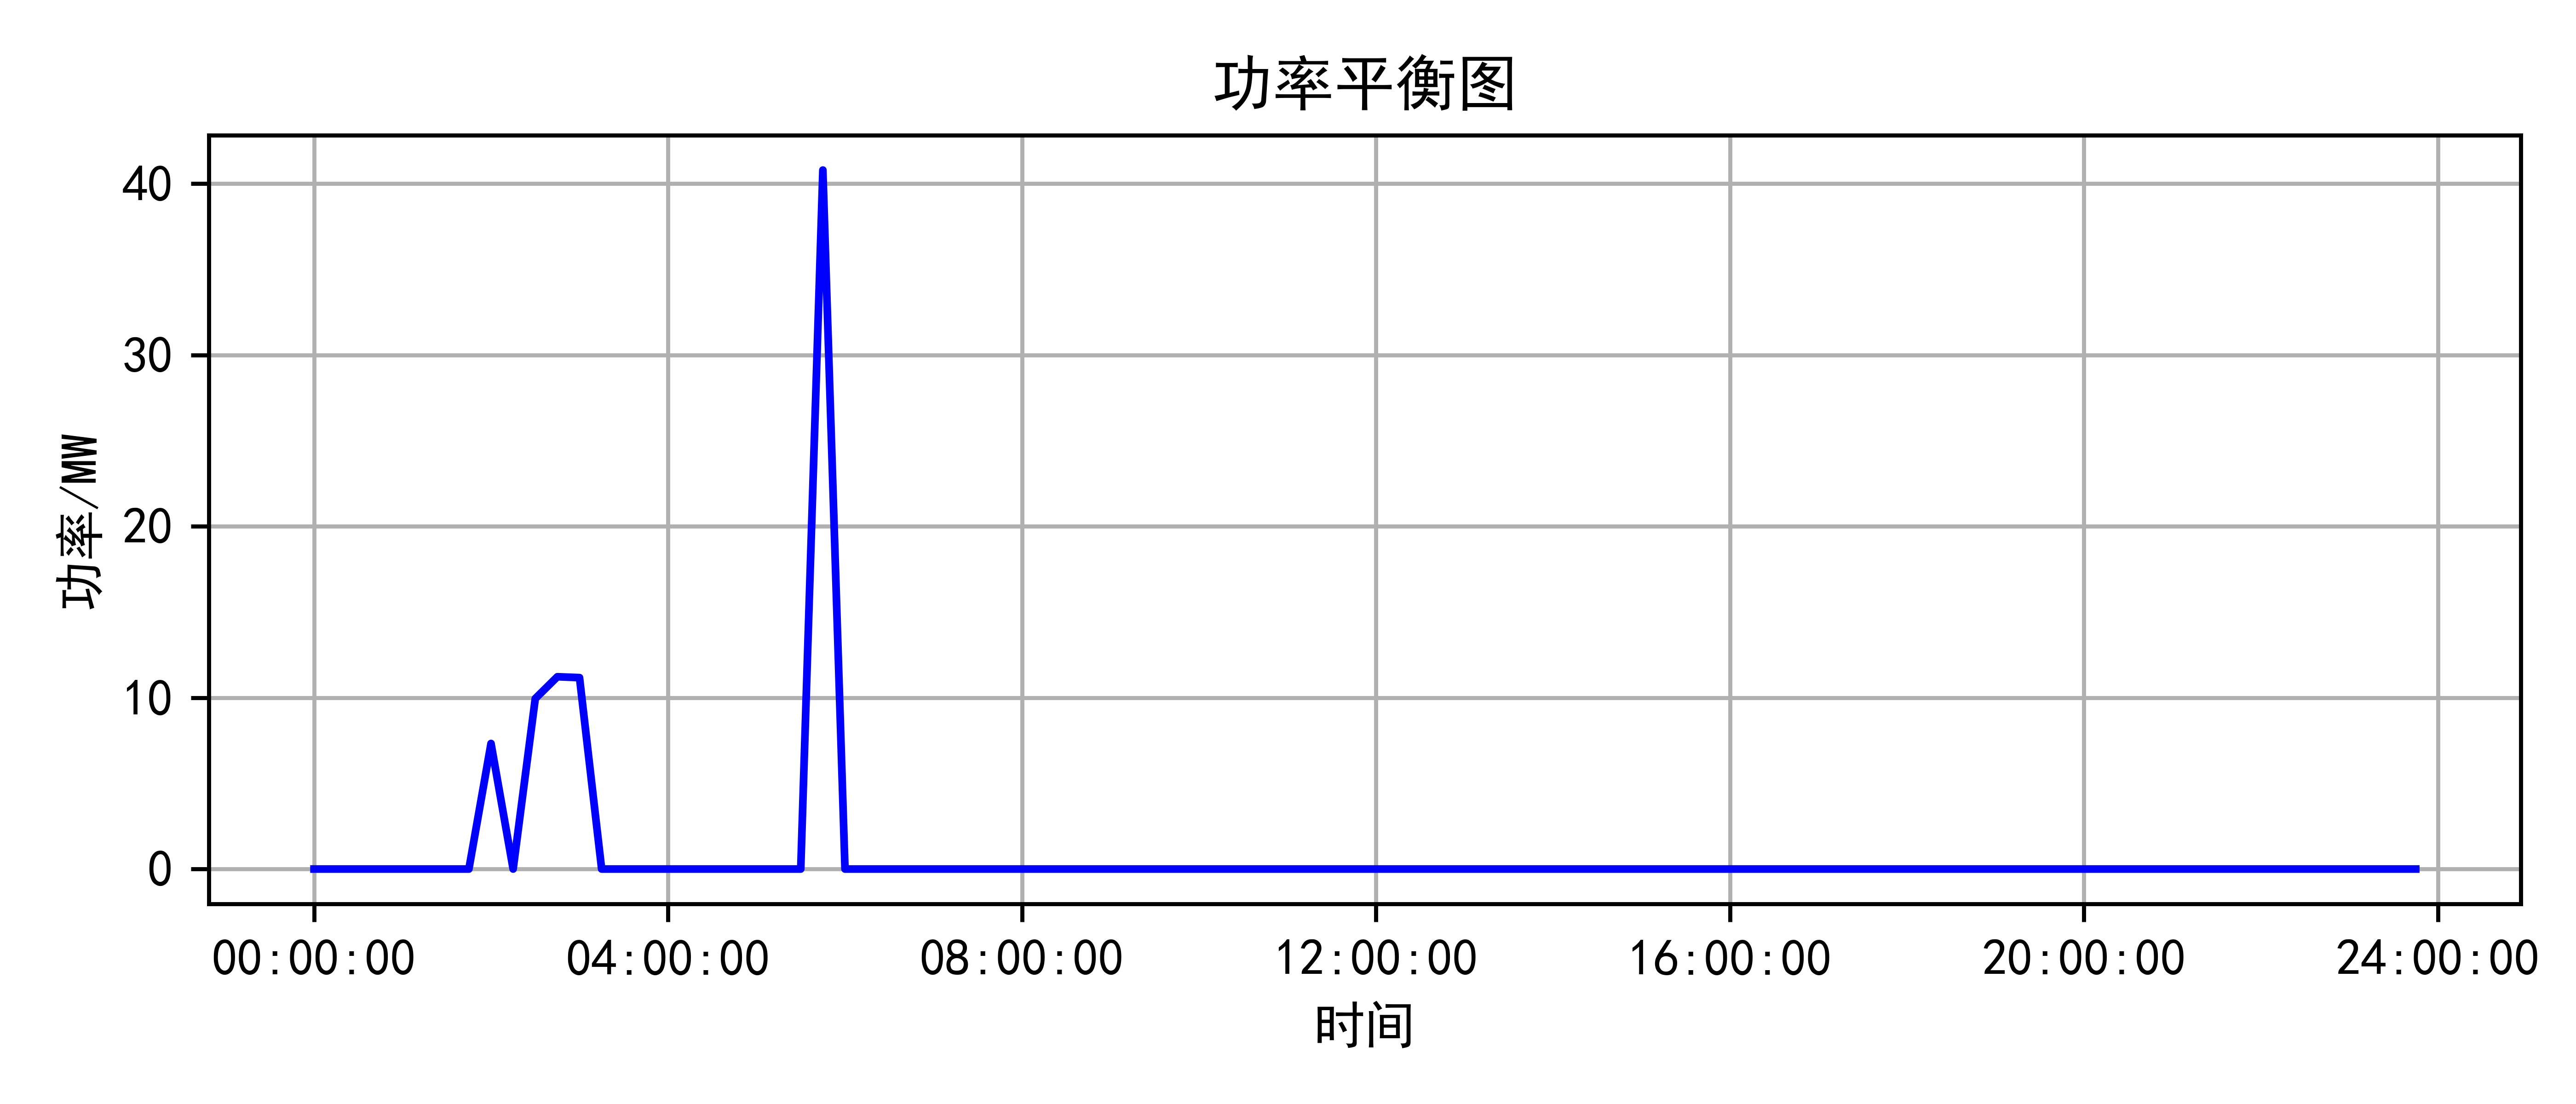
\includegraphics[width=1\linewidth]{figures/第二题:功率平衡图}
		\caption{功率平衡图}
		\label{fig:}
	\end{figure}
	
	从图中可以看到,功率平衡存在$ \texttt{系统总功率}\geq \texttt{负荷所需功率}$的情况,因此会导致出现弃风现象。
	
	 \newpage
\section{600MW风机替代机组2后系统功率平衡变化情况分析}
\subsection{本题求解过程}
\subsubsection{本题求解流程}
\begin{figure}[H]  
	\centering
	
	\scriptsize  
	
	%像素点,用于连接转移线
	\begin{tikzpicture}[node distance=2cm]
		%定义流程图具体形状
		\node (start1) [startstop] {制定火电机组最优发电计划};
		\node (in1) [process, below of=start1] {计算弃风功率$ P_{wind\ loss} $的曲线};
		\node (pro1) [process, below of=in1,] {将弃风功率在时间上进行积分,得到弃风量};
		\node (in2) [process, below of=pro1] {计算失负荷功率$ P_{load\ loss} $的曲线};
		\node (pro2) [process, below of=in2,] {将失负荷功率在时间上进行积分,得到失负荷量};
		\node (stop1) [startstop, below of=pro2]{得到结果};
		
		%连接具体形状
		\draw [arrow](start1) -- (in1);
		\draw [arrow](in1) --  (pro1);
		\draw [arrow](pro1) --  (in2);
		\draw [arrow](in2) --  (pro2);
		\draw [arrow](pro2) --  (stop1);
	\end{tikzpicture}
	\caption{第三题求解流程}
	\label{dthz}
\end{figure} 
	上图是第三题求解的流程图,我们首先通过等微增率算法计算制定火电机组1、3的最优发电计划,然后再计算弃风功率$ P_{wind\ loss} $的曲线,接着将弃风功率在时间上进行积分,得到弃风量,而后再计算失负荷功率$ P_{load\ loss} $的曲线,再而后将失负荷功率在时间上进行积分,得到失负荷量,最后得到结果。

\subsubsection{火电机组最优功率}
本题中,风机替代了机组2,根据\textbf{节\ref{sjzdwzl}}中双机组最优功率求解可以计算出机组1、3的最优功率发电曲线。



\subsubsection{计算风机功率缺额}
通过节\ref{jsqflsfhl}中的函数\textbf{get\_wind\_loss}可以计算系统机组总功率与负荷功率之差,其中差值的最小值即为系统的风机功率缺额。

\subsection{计算结果}
缺额的风电装机容量为:47.67MW,即需要增加接入风机装机容量为:47.67MW。弃风电量为:268.861MWh。


	功率平衡变化如下图:
% TODO: \usepackage{graphicx} required
\begin{figure}[H]
	\centering
	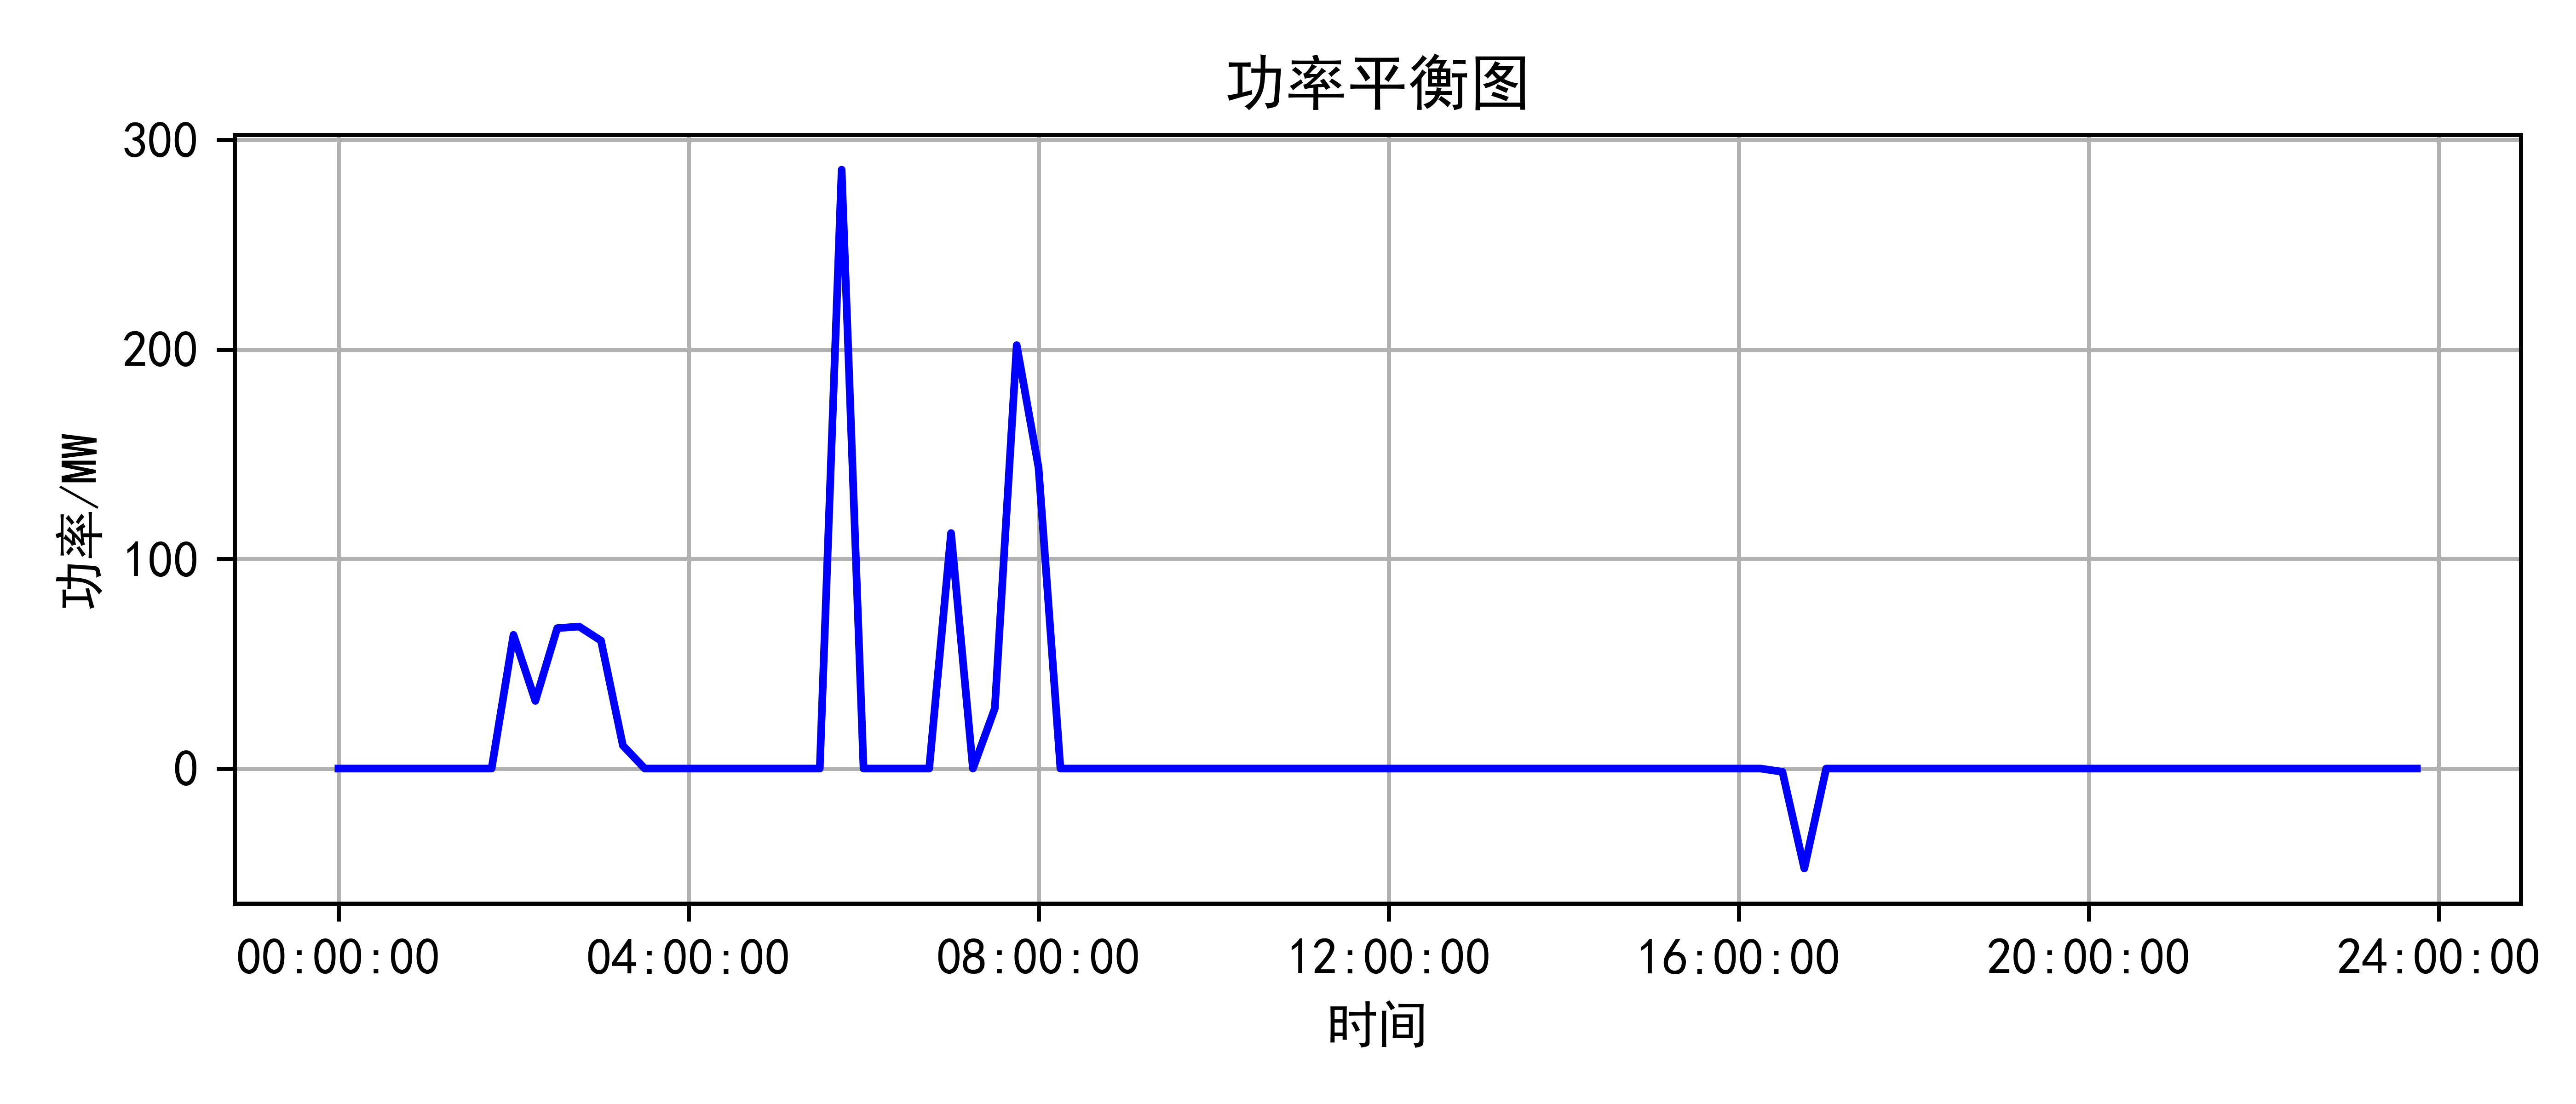
\includegraphics[width=1\linewidth]{figures/第三题:功率平衡图}
	\caption{功率平衡图}
	\label{fig:}
\end{figure}

	从图中可以看到,功率平衡存在$ \texttt{系统总功率}\geq \texttt{负荷所需功率}$的情况,因此会导致出现弃风现象。
	
	同时也存在$ \texttt{系统总功率}\leq \texttt{负荷所需功率}$的情况,此时会导致出现失负荷现象。
	
	 \newpage
	\section{针对上述两种替代情景计算相关数据}
	\subsection{本题求解过程}
	\subsubsection{本题求解流程}
	\begin{figure}[H]  
		\centering
		
		\scriptsize  
		
		%像素点,用于连接转移线
		\begin{tikzpicture}[node distance=2cm]
			%定义流程图具体形状
			\node (start1) [startstop] {制定火电机组最优发电计划};
			\node (in1) [process, below of=start1] {计算弃风功率$ P_{wind\ loss} $曲线};
			\node (pro1) [process, below of=in1,] {将弃风功率在时间上进行积分,得到弃风量};
			\node (pro4) [process, below of=pro1,] {计算弃风损失};
			\node (in2) [process, below of=pro4] {计算失负荷功率$ P_{load\ loss} $曲线};
			\node (pro2) [process, below of=in2,] {将失负荷功率在时间上进行积分,得到失负荷量};
			\node (pro3) [process, below of=pro2,] {计算失负荷损失};
			\node (pro5) [process, below of=pro3,] {计算火电成本};
			\node (stop1) [startstop, below of=pro5]{得到结果};
			
			%连接具体形状
			\draw [arrow](start1) -- (in1);
			\draw [arrow](in1) --  (pro1);
			\draw [arrow](pro1) --  (pro4);
			\draw [arrow](pro4) --  (in2);
			\draw [arrow](in2) --  (pro2);
			\draw [arrow](pro2) --  (pro3);
			\draw [arrow](pro3) --  (pro5);
			\draw [arrow](pro5) --  (stop1);
		\end{tikzpicture}
		\caption{第四题求解流程}
		\label{dthz}
	\end{figure} 
	上图是第四题求解的流程图,我们先通过等微增率算法计算得出火电机组最优发电计划以及计算出弃风功率$ P_{wind\ loss} $的曲线,然后将弃风功率在时间上进行积分,得到弃风量,结合以上结果计算出弃风损失。再然后我们计算失负荷功率$ P_{load\ loss} $曲线,同时将失负荷功率在时间上进行积分,得到失负荷量。之后,我们计算失负荷损失以及火电成本。最后得出结果。
	\subsection{对于300MW风机替代机组3}
	原始数据可以直接使用第二题的结果。
	
	从第二题存储的运行数据中取出差值,调用函数\textbf{get\_wind\_load}计算出弃风量,从而计算出弃风损失。由于替代机组3的情况下没有失负荷,因此不需要计算失负荷量。
	
	火电成本可以根据第一题方式进行计算。将不同的碳捕集单价放入函数中即可得到不同的系统运行单价。
	
	\subsubsection*{计算结果}
	% Please add the following required packages to your document preamble:
	% \usepackage{multirow}
	% \usepackage{graphicx}
	\begin{table}[H]
		\centering
		\caption{风电装机300MW替代机组3时系统相关指标统计}
		\label{tab:my-table}
		\resizebox{\textwidth}{!}{%
			\begin{tabular}{lllllllll}
				\toprule[1.5pt]
				\multicolumn{1}{c}{\multirow{2}{*}{\begin{tabular}[c]{@{}c@{}}碳捕集\\ 成本\\ (元/t)\end{tabular}}} &
				\multicolumn{1}{c}{\multirow{2}{*}{\begin{tabular}[c]{@{}c@{}}火电运行\\ 成本\\ (万元)\end{tabular}}} &
				\multicolumn{1}{c}{\multirow{2}{*}{\begin{tabular}[c]{@{}c@{}}碳捕集\\ 成本\\ (万元)\end{tabular}}} &
				\multicolumn{1}{c}{\multirow{2}{*}{\begin{tabular}[c]{@{}c@{}}风电运维\\ 成本\\ (万元)\end{tabular}}} &
				\multicolumn{2}{c}{弃风损失} &
				\multicolumn{2}{c}{失负荷损失} &
				\multicolumn{1}{c}{\multirow{2}{*}{\begin{tabular}[c]{@{}c@{}}单位供\\ 电成本\\ (元/KWh)\end{tabular}}} \\ \cline{5-8}
				\multicolumn{1}{c}{} &
				\multicolumn{1}{c}{} &
				\multicolumn{1}{c}{} &
				\multicolumn{1}{c}{} &
				\begin{tabular}[c]{@{}l@{}}弃风电量\\ (MW)\end{tabular} &
				\begin{tabular}[c]{@{}l@{}}弃风损失\\ (万元)\end{tabular} &
				\begin{tabular}[c]{@{}l@{}}失负荷电\\ 量(MW)\end{tabular} &
				\begin{tabular}[c]{@{}l@{}}失负荷损失\\ (万元)\end{tabular} &
				\multicolumn{1}{c}{} \\ \midrule[1pt]
				0.000   & 201.892 & 0.000  & 9.115 & 20.113 & 0.603 & 0.000 & 0.000 & 0.136 \\
				60.000  & 201.892 & 58.939 & 9.115 & 20.113 & 0.603 & 0.000 & 0.000 & 0.174 \\
				80.000  & 201.892 & 78.585 & 9.115 & 20.113 & 0.603 & 0.000 & 0.000 & 0.187 \\
				100.000 & 201.892 & 98.232 & 9.115 & 20.113 & 0.603 & 0.000 & 0.000 & 0.200 \\ \bottomrule[1.5pt]
			\end{tabular}%
		}
	\end{table}
	\subsection{对于600MW风机替代机组2}
	原始数据可以直接使用第三题的结果。
	
	从第三题存储的运行数据中取出差值。调用函数\textbf{get\_wind\_load}计算出弃风量,从而计算出弃风损失。调用函数\textbf{get\_loss\_load}计算出失负荷量,从而计算出失负荷损失。
	
	
	火电成本可以根据第一题方式进行计算。将不同的碳捕集单价放入函数中即可得到不同的系统运行单价。
	\subsubsection*{计算结果}
	% Please add the following required packages to your document preamble:
	% \usepackage{multirow}
	% \usepackage{graphicx}
	\begin{table}[H]
		\centering
		\caption{风电装机600MW替代机组2时系统相关指标统计}
		\label{tab:my-table}
		\resizebox{\textwidth}{!}{%
			\begin{tabular}{lllllllll}
				\toprule[1.5pt]
				\multicolumn{1}{c}{\multirow{2}{*}{\begin{tabular}[c]{@{}c@{}}碳捕集\\ 成本\\ (元/t)\end{tabular}}} &
				\multicolumn{1}{c}{\multirow{2}{*}{\begin{tabular}[c]{@{}c@{}}火电运行\\ 成本\\ (万元)\end{tabular}}} &
				\multicolumn{1}{c}{\multirow{2}{*}{\begin{tabular}[c]{@{}c@{}}碳捕集\\ 成本\\ (万元)\end{tabular}}} &
				\multicolumn{1}{c}{\multirow{2}{*}{\begin{tabular}[c]{@{}c@{}}风电运维\\ 成本\\ (万元)\end{tabular}}} &
				\multicolumn{2}{c}{弃风损失} &
				\multicolumn{2}{c}{失负荷损失} &
				\multicolumn{1}{c}{\multirow{2}{*}{\begin{tabular}[c]{@{}c@{}}单位供\\ 电成本\\ (元/KWh)\end{tabular}}} \\ \cline{5-8}
				\multicolumn{1}{c}{} &
				\multicolumn{1}{c}{} &
				\multicolumn{1}{c}{} &
				\multicolumn{1}{c}{} &
				\begin{tabular}[c]{@{}l@{}}弃风电量\\ (MW)\end{tabular} &
				\begin{tabular}[c]{@{}l@{}}弃风损失\\ (万元)\end{tabular} &
				\begin{tabular}[c]{@{}l@{}}失负荷电\\ 量(MW)\end{tabular} &
				\begin{tabular}[c]{@{}l@{}}失负荷损失\\ (万元)\end{tabular} &
				\multicolumn{1}{c}{} \\ \midrule[1pt]
				0.000                       & 167.326 & 0.000  & 18.230 & 268.861 & 8.066 & 12.304 & 9.843 & 0.131 \\
				60.000                      & 167.326 & 50.906 & 18.230 & 268.861 & 8.066 & 12.304 & 9.843 & 0.164 \\
				80.000 & 167.326 & 67.875 & 18.230 & 268.861 & 8.066 & 12.304 & 9.843 & 0.175 \\
				100.000                     & 167.326 & 84.844 & 18.230 & 268.861 & 8.066 & 12.304 & 9.843 & 0.186 \\ \bottomrule[1.5pt]
			\end{tabular}%
		}
	\end{table}

	\subsection{代码封装以及实现}
	函数\textbf{get\_loss\_load}存放在\textbf{附录B-Python程序源代码-第四题-600MW风电替代机组2-第四题:计算费用-600MW替代.py}中。
	
	 \newpage
	\section{计算900MW替代2,3机组相关数据}
	\subsection{本题求解过程}\label{diwuti}
	\subsubsection{本题求解流程}
	\begin{figure}[H]  
		\centering
		
		\scriptsize  
		
		%像素点,用于连接转移线
		\begin{tikzpicture}[node distance=2cm]
			%定义流程图具体形状
			\node (start1) [startstop] {计算机组1功率$ P $的曲线};
			\node (in1) [process, below of=start1] {计算弃风功率$ P_{wind\ loss} $的曲线};
			\node (pro1) [process, below of=in1,] {将弃风功率在时间上进行积分,得到弃风量};
			\node (pro4) [process, below of=pro1,] {计算弃风损失};
			\node (in2) [process, below of=pro4] {计算失负荷功率$ P_{load\ loss} $的曲线};
			\node (pro2) [process, below of=in2,] {将失负荷功率在时间上进行积分,得到失负荷量};
			\node (pro3) [process, below of=pro2,] {计算失负荷损失};
			\node (pro5) [process, below of=pro3,] {计算火电成本};
			
			\node (stop1) [startstop, below of=pro5]{计算储能容量、储能功率和储能成本};
			\node (stop2) [startstop, below of=stop1]{得到结果};
			%连接具体形状
			\draw [arrow](start1) -- (in1);
			\draw [arrow](in1) --  (pro1);
			\draw [arrow](pro1) --  (pro4);
			\draw [arrow](pro4) --  (in2);
			\draw [arrow](in2) --  (pro2);
			\draw [arrow](pro2) --  (pro3);
			\draw [arrow](pro3) --  (pro5);
			\draw [arrow](pro5) --  (stop1);
			\draw [arrow](stop1) --  (stop2);
		\end{tikzpicture}
		\caption{第五题求解流程}
		\label{dthz}
	\end{figure} 
    上图是第五题求解的流程图,我们先计算机组1功率$ P $以及计算弃风功率$ P_{wind\ loss} $的曲线,然后将弃风功率在时间上进行积分,得到弃风量。然后计算弃风损失以及失负荷功率$ P_{load\ loss} $的曲线,将失负荷功率在时间上进行积分,得到失负荷量。在之后我们计算失负荷损失,火电成本以及储能成本。最后得出结果。
	
	\subsubsection{机组功率}
	在本题中,由于风电替代了机组2、3,因此机组1功率可以用$ \texttt{目标功率} -\texttt{风电功率}$进行计算。但计算的同时需要关注机组出力上下限问题,因此需要使用函数\textbf{judge}进行辅助判断。
	
	\subsubsection{储能成本}
	储能成本分为两大类:投资成本和运维成本。
	
	\textbf{1)投资成本}
	
	投资成本又分为单位功率成本和单位能量成本。其中单位功率成本指:每建设1KW功率的储能系统所需的成本;单位能量成本指:所建设储能系统的容量每增加1KWh所需要的成本。
	
	由于投资成本是一次性费用,因此需要将其均摊才能计入系统总成本计算中。此处储能系统的设计寿命是10年,因此所计算的储能成本应$ /\texttt{10年}/\texttt{365天} $,所得结果方可使用。
	
	\textbf{2)运维成本}
	
	单位运维成本指储能系统每放出1KWh所需的运维费用,因此总运维费用可以用$ \texttt{总放电量}\times \texttt{单位运维成本}$进行计算。
	
	\subsubsection{储能容量与功率}
	对于本题需要的储存容量和储能功率,其计算方式如下:
	
	\begin{enumerate}
		\item 计算系统最大功率缺额
		\item $ \texttt{所需储能功率}\geq \texttt{最大功率缺额}\times \texttt{储能效率}$
		\item 计算系统最大容量缺额
		\item  $ \texttt{所需储存容量} \geq \texttt{最大容量缺额}\times \texttt{储能效率}$
	\end{enumerate}
	
	
	\subsection{计算结果}
	
	风电装机900MW、替代机组2、3时,失负荷电量215.891MWh,最大失负荷功率为146.505MW,需要配备最小储能容量为162.783MWh。考虑碳捕集成本60元/吨,此时单位供电成本为0.147元/KWh。
	
	
	 \newpage
	\section{探究风电接入对系统供电的影响}
	
	根据节1.6中表1 风电电量占比为0时系统相关指标统计可得,火电运行成本不随着单位碳捕集成本的改变而改变,为244.573万元。同时,当单位碳捕集成本逐渐增大时,碳捕集成本、总发电成本以及单位供电成本都在不断增加。
	
	风电装机 300MW、替代机组 3 时,根据节2.6中图5 功率平衡图可得,系统功率在2时到4时期间以及6时左右经历了两次陡增,破坏了原有的功率平衡,风功率过剩,面临保消纳的问题,对系统可靠供电造成挑战。同时将节4.2中表2风电装机 300MW 替代机组 3 时系统相关指标统计与节1.6中表1 风电电量占比为0时系统相关指标统计的数据进行比对,发现:风电装机300MW替代机组3,单位碳捕集成本相同时,单位供电成本均得到了13\%左右的下降。
	
	风电装机 600MW、替代机组 2 时,根据节3.2中图7 功率平衡图可得,系统功率在2时到4时期间、6时到8时期间、系统功率陡增,风功率过剩,面临保消纳的问题。17时左右系统功率骤降,供应不足,系统面临着保供应的问题。二者都对系统可靠用电造成挑战。同时将节4.3中表3风电装机 600MW 替代机组 2 时系统相关指标统计与节1.6中表1 风电电量占比为0时系统相关指标统计的数据进行比对,发现:风电装机600MW替代机组2,单位碳捕集成本相同时,单位供电成本均得到了17\%左右的下降。
	
	综合上述分析可得,风电替代容量的递增会破坏系统的功率平衡,对系统的供电能力带来了不稳定性与波动性。但同时为保障可靠供电,系统单位供电成本会随着风电替代容量的递增而减少。
	
	 \newpage
	\section{风电装机1200MW替代机组2,3时对功率平衡的分析}
	
	\subsection{功率平衡}\label{功率平衡}
	本节功率平衡计算与第三题中功率平衡算法相同。下面是其结果:
	
	% TODO: \usepackage{graphicx} required
	\begin{figure}[H]
		\centering
		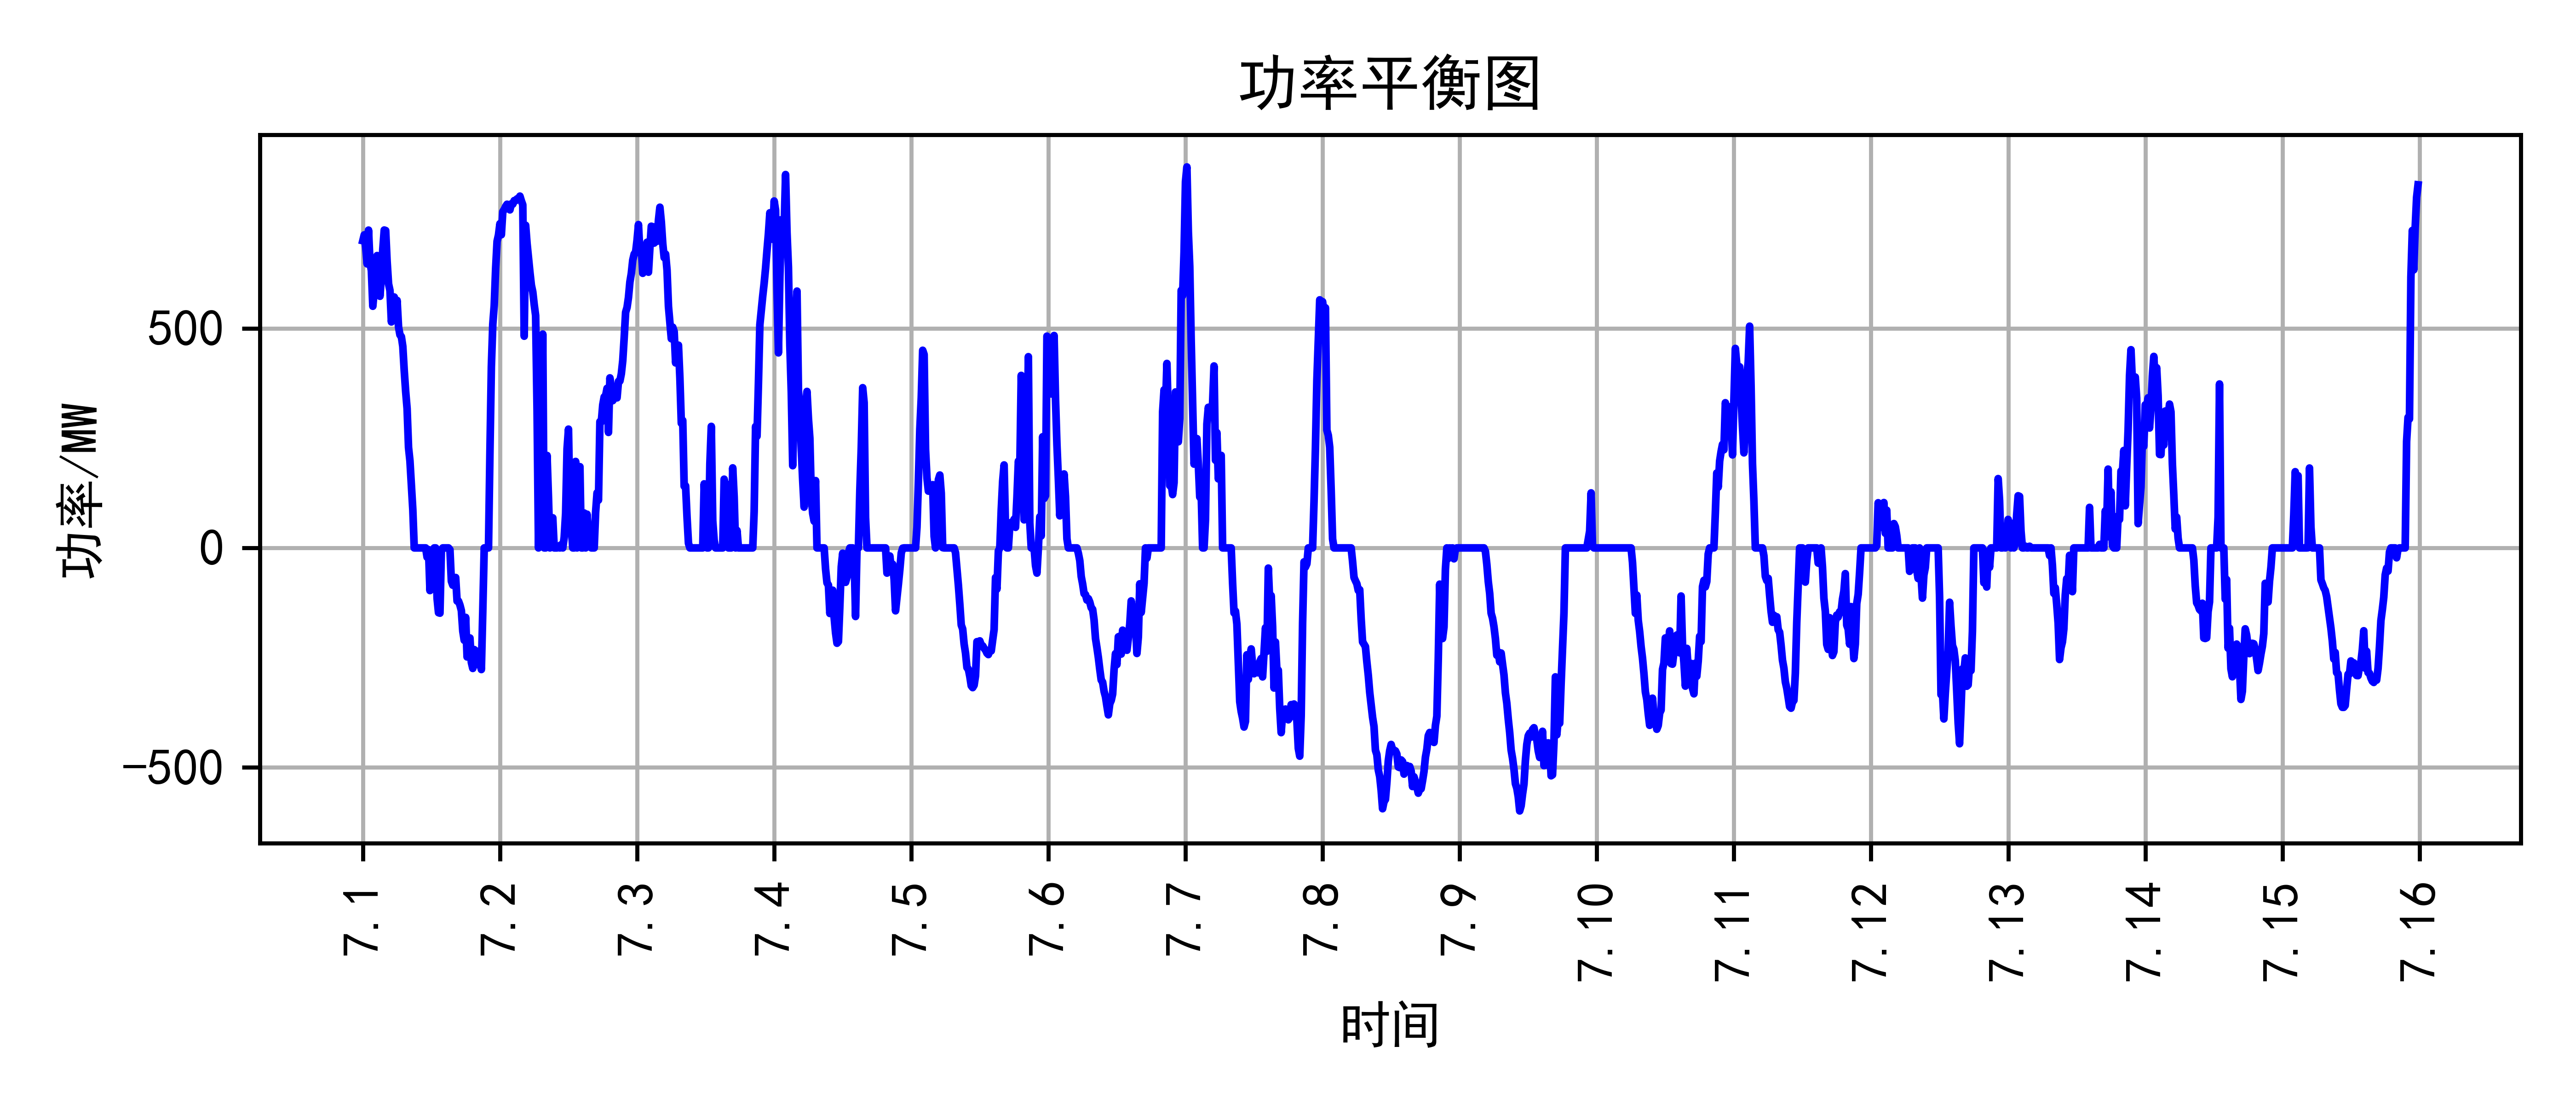
\includegraphics[width=1\linewidth]{figures/第七题:功率平衡图}
		\caption{功率平衡图}
		\label{fig:}
	\end{figure}
	
	
	
	\subsection{遗传算法}
	
	
	遗传算法(Genetic Algorithm, GA)是模拟达尔文生物进化论的自然选择和遗传学机理的生物进化过程的计算模型,是一种通过模拟自然进化过程搜索最优解的方法\cite{2}。
	
	% TODO: \usepackage{graphicx} required
	\begin{figure}[H]
		\centering
		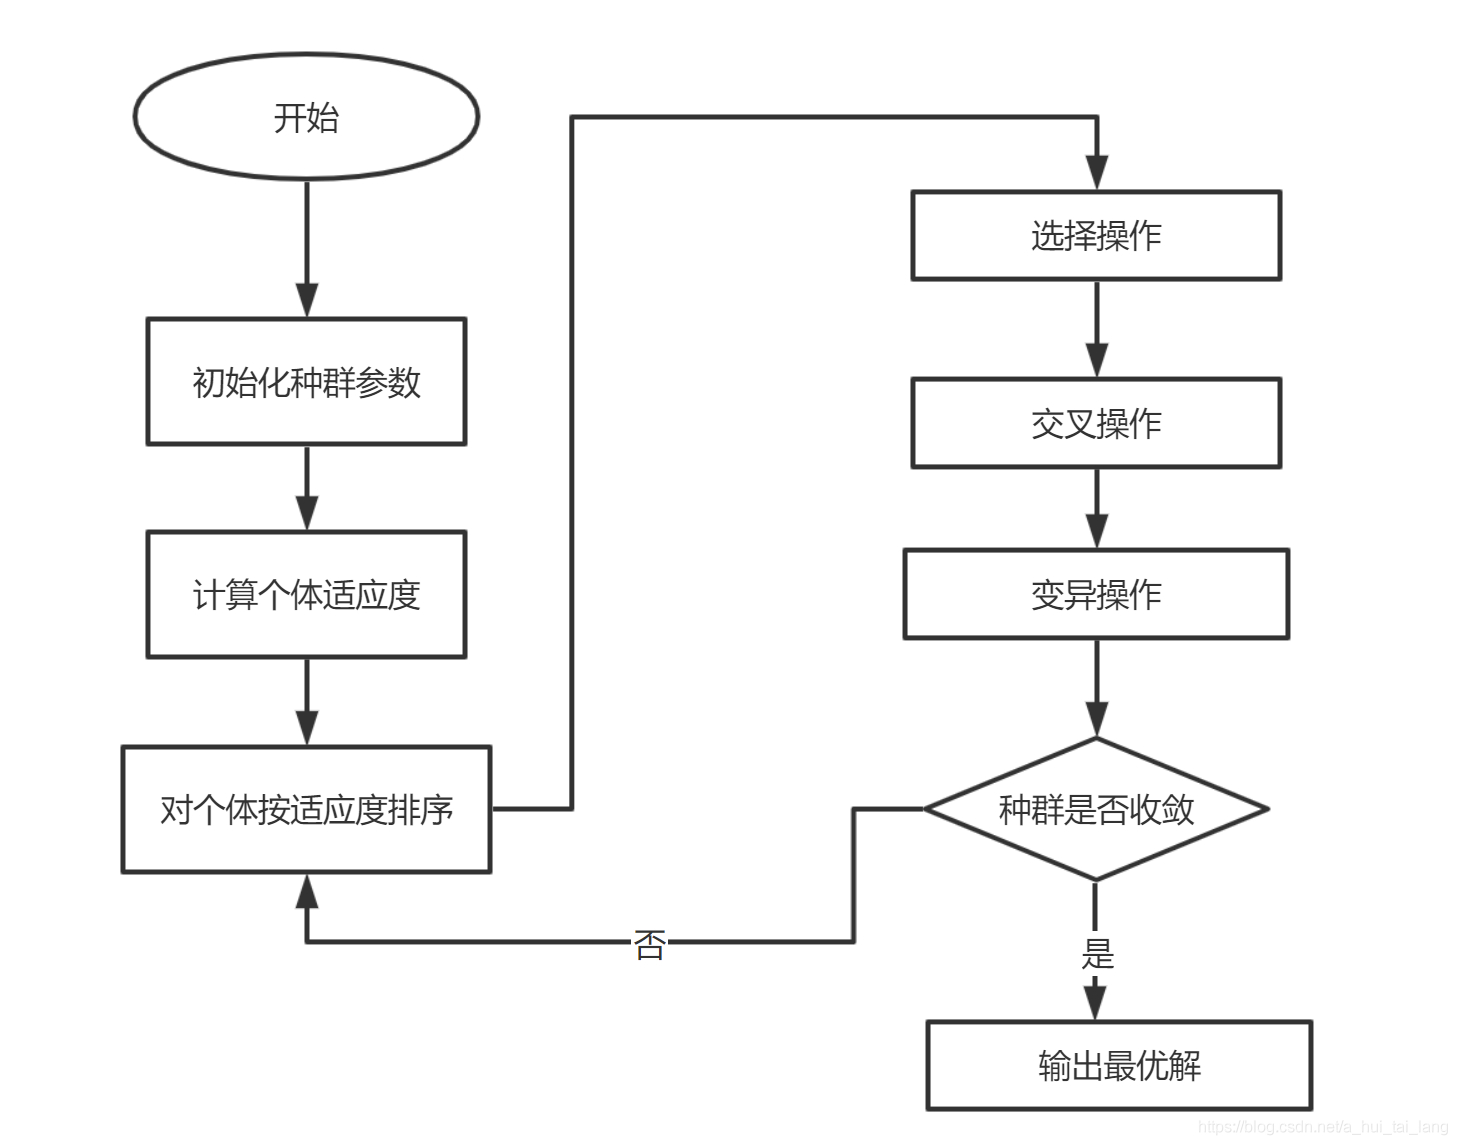
\includegraphics[width=0.7\linewidth]{figures/screenshot001}
		\caption{遗传算法流程}
		\label{fig:screenshot001}
	\end{figure}
	
	本节通过该算法进行最优解计算。
	
	\subsection{系统优化}
	\subsubsection{优化目标}
	系统优化目标为系统供电成本$ C $(元/KWh)。即:
	\begin{equation}\label{key}
	C=f(C_{es},P_{es})
	\end{equation}

	其中:$ C_{es} $为储能系统的容量,$ P_{es} $为储能系统的功率。
	
	目标函数使用使用第五题中的算法,其详细过程见节\ref{diwuti}。
	\subsubsection{优化变量}
	
	需要优化的变量有两个:储能系统的容量$ C_{es} $和储能系统的功率$ P_{es} $。根据节\ref{功率平衡}结果,最大功率缺额约为600MW,最大容量缺额为150MWh。因此,我们可以得到以下的约束条件:
	
	\begin{equation}\label{ystj}
		\left\{\begin{matrix}
		0\leq P_{es}\leq 600\\
		0\leq C_{es}\leq 150
		\end{matrix}\right.
	\end{equation}
	
	\subsubsection{遗传算法求解}\label{yc}
	根据约束条件,即式\ref{ystj},可以得到:对于单个变量而言,若精确到小数点后5为,则应有的染色体数目为20。
	
	因此,本节中,我们使每个个体为40条染色体,其中前20代表储能系统的容量$ C_{es} $,后20为储能系统的功率$ P_{es} $;种群共有50个个体。
	
	
	\subsubsection{遗传算法结果(碳捕集成本为0元/吨)}
	使用参数为:$ c=0.4\texttt{,}m=0.02\texttt{,}iter\_num=500 $,迭代过程如下图:
	% TODO: \usepackage{graphicx} required
	\begin{figure}[H]
		\centering
		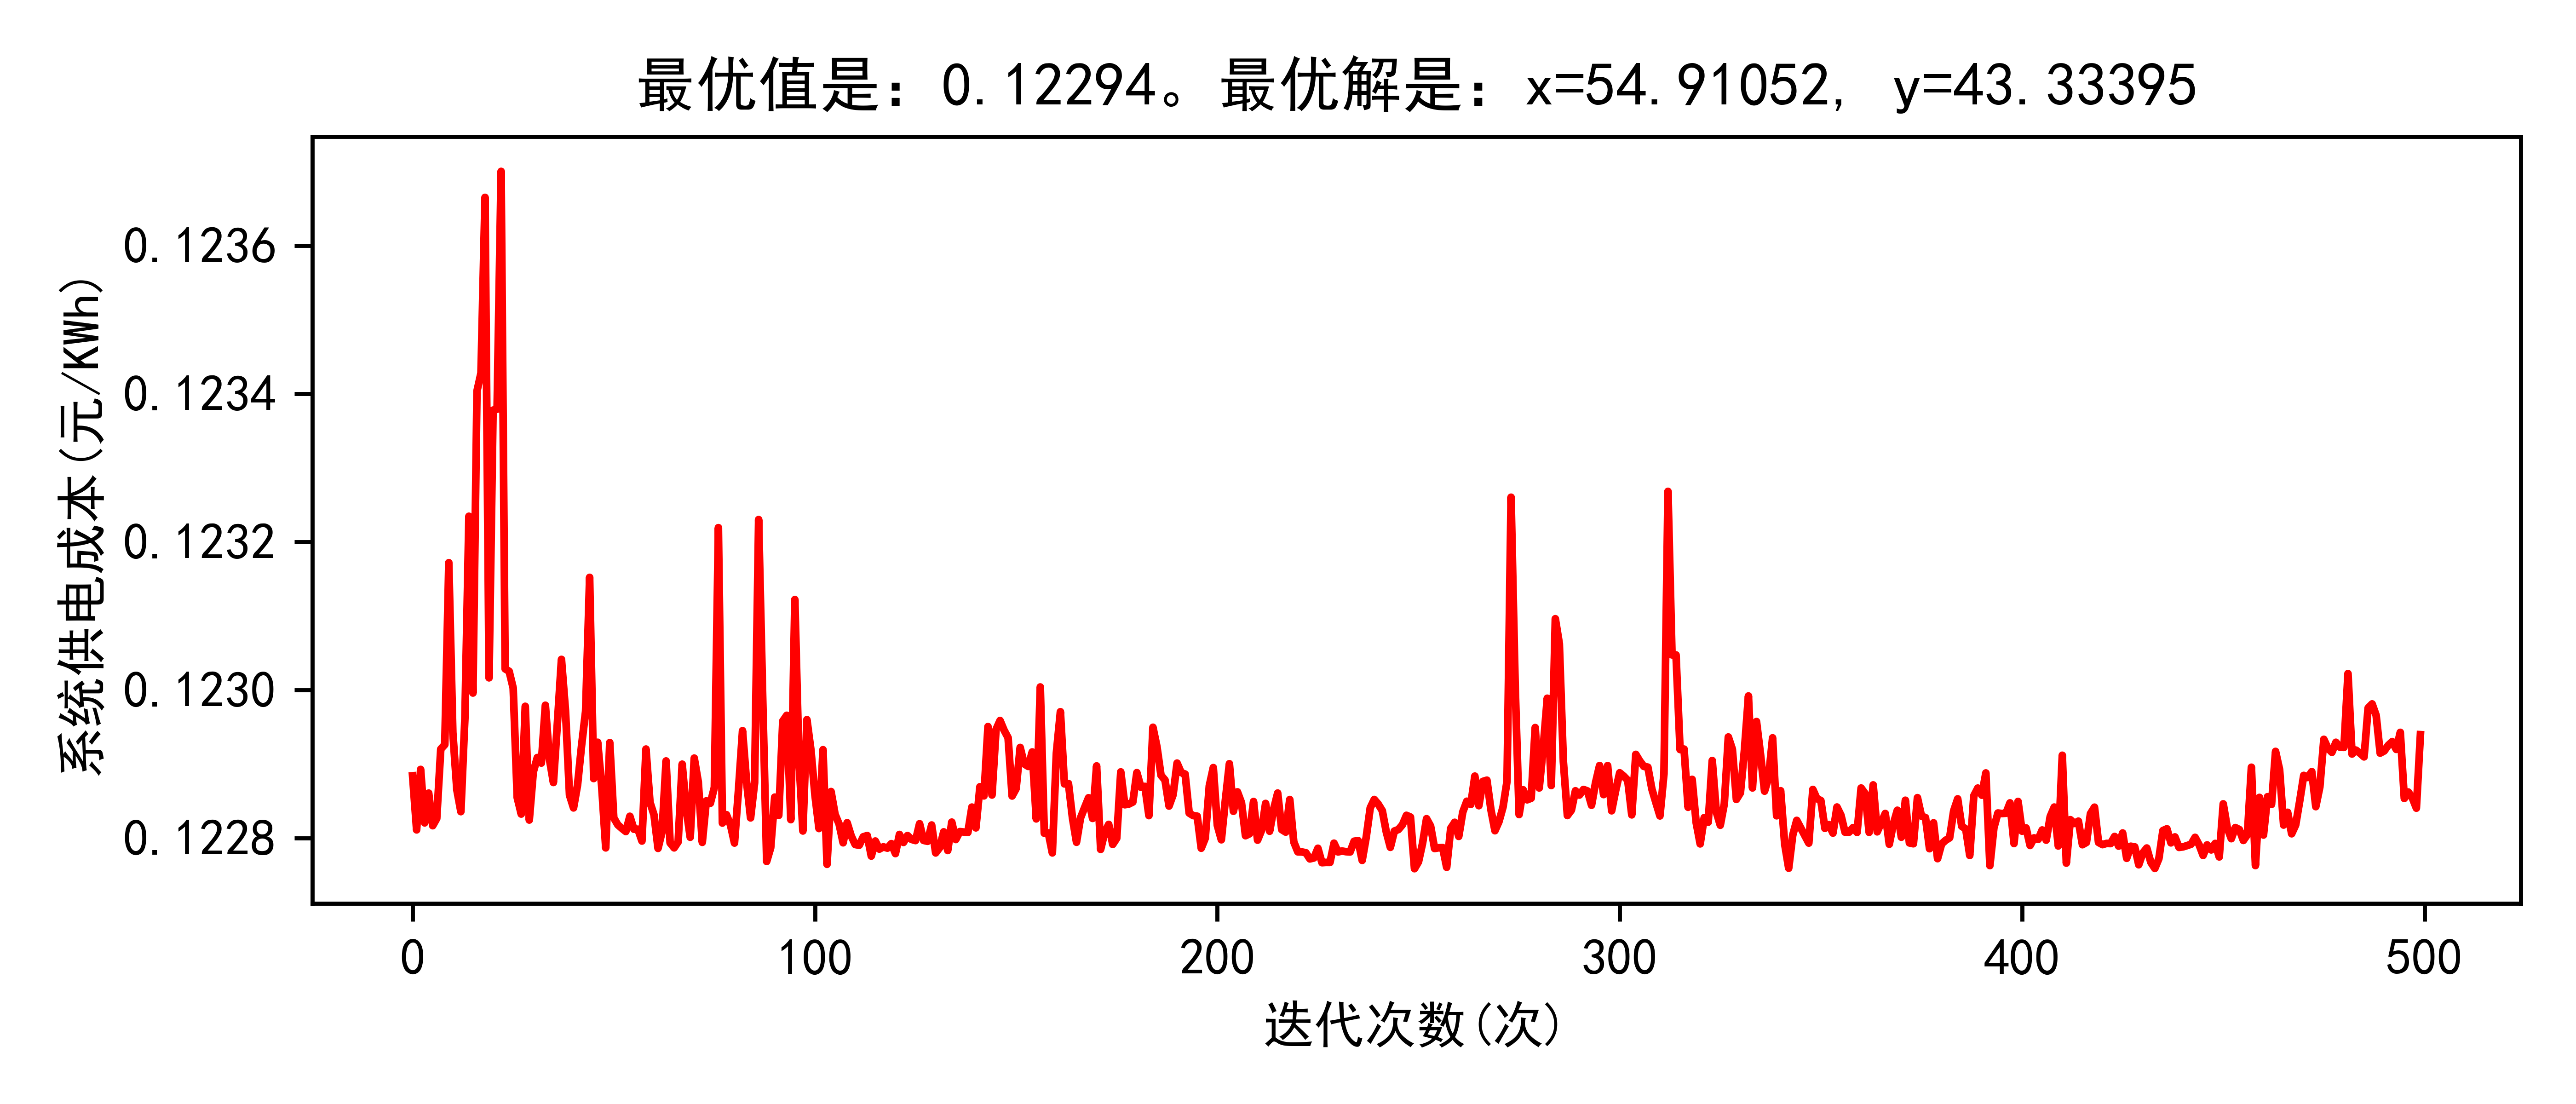
\includegraphics[width=1\linewidth]{figures/交叉:0.4,变异:0.02,迭代次数:500,成本:0}
		\caption{遗传算法结果}
		\label{fig:0}
	\end{figure}
	
	可以发现,当储能容量为54.911MWH,储能功率为43.334MW时,所得的系统供电成本最低,为0.12294元/KWh。
	
	\subsubsection{其他情况}
	其他碳捕集成本下的情况如下表所示:
	
	% Please add the following required packages to your document preamble:
	% \usepackage{graphicx}
	\begin{table}[H]
		\centering
		\caption{不同碳捕集成本下的储能最优解}
		\label{tab:my-table}
		\begin{tabular}{llll}
		\toprule[1.5pt]
		\begin{tabular}[c]{@{}l@{}}碳捕集成本\\ (元/吨)\end{tabular} &
		\begin{tabular}[c]{@{}l@{}}储能容量\\ (MWh)\end{tabular} &
		\begin{tabular}[c]{@{}l@{}}储能功率\\ (MW)\end{tabular} &
		\begin{tabular}[c]{@{}l@{}}系统供电成本\\ (元/KWh)\end{tabular} \\\midrule[1pt]
		0   & 54.911  & 43.334 & 0.12294 \\
		60  & 127.633 & 40.916 & 0.14501 \\
		80  & 45.568  & 74.929 & 0.15209 \\
		100 & 45.332  & 19.703 & 0.15934 \\ \bottomrule[1.5pt]
	\end{tabular}%
	\end{table}

	\begin{table}[H]
	\centering
	\caption{风电装机1200MW替代机组2,3时供电成本}
	\label{tab:my-table}
	\begin{tabular}{llll}
		\toprule[1.5pt]
		\begin{tabular}[c]{@{}l@{}}碳捕集成本\\ (元/吨)\end{tabular} &
		\begin{tabular}[c]{@{}l@{}}储能容量\\ (MWh)\end{tabular} &
		\begin{tabular}[c]{@{}l@{}}储能功率\\ (MW)\end{tabular} &
		\begin{tabular}[c]{@{}l@{}}系统供电成本\\ (元/KWh)\end{tabular} \\\midrule[1pt]
	    0   & 0  & 0 & 0.12276 \\
	    60  & 0 & 0 & 0.14462 \\
	    80  & 0  & 0 & 0.15191 \\
	    100 & 0  & 0 & 0.15920 \\ \bottomrule[1.5pt]
	\end{tabular}%
	\end{table}

由于不同各种储能装置由于具有对功率和能量的时间迁移能力,是充分改善现有的功率不平衡的有效手段。结合表4 表5的数据,不同单位碳捕集成本下,在储能最优解时,系统供电成本与同情况下储能未接入时系统供电成本所差无几。在经济性上,本方案具有一定的可行性。同时由于储能元件的自身的特性,本方案也具有显著的有效性。

	\subsection{代码的封装及实现}
	将节\ref{yc}的遗传算法封装为函数\textbf{ga},其传入参数为交叉概率$ c $,变异概率$ m $,迭代次数$ iter\_num $。
	
	函数\textbf{ga}的详细代码在\textbf{附录B-Python程序源代码-第七题-第七题:遗传算法求最优解.py}中。
	
	
	 \newpage
	\section{结论}
	问题一:碳捕集成本为0时,单位供电成本为0.158元/KWh;碳捕集成本为60时,单位供电成本为0.202元/KWh;碳捕集成本为80时,单位供电成本为0.216元/KWh;碳捕集成本为100时,单位供电成本为0.231元/KWh。
	
	问题二:风电装机300MW替代机组3时,功率平衡存在$ \texttt{系统总功率}\geq \texttt{负荷所需功率}$的情况,弃风电量为20.113MWh,为减少弃风又不失负荷风电装机容量需要降低40.789MW。
	
	问题三:风电装机600MW替代机组2时,功率平衡存在$ \texttt{系统总功率}\geq \texttt{负荷所需功率}$的情况,因此会导致出现弃风现象。同时也存在$ \texttt{系统总功率}\leq \texttt{负荷所需功率}$的情况,此时会导致出现失负荷现象。为不失负荷,风电装机容量要增加47.67MW。
	
	问题四:对于风电装机300MW替代机组3时,碳捕集成本为0时,单位供电成本为0.136元/KWh;碳捕集成本为60时,单位供电成本为0.174元/KWh;碳捕集成本为80时,单位供电成本为0.187元/KWh;碳捕集成本为100时,单位供电成本为0.200元/KWh。对于风电装机600MW替代机组2时,碳捕集成本为0时,单位供电成本为0.131元/KWh;碳捕集成本为60时,单位供电成本为0.164元/KWh;碳捕集成本为80时,单位供电成本为0.175元/KWh;碳捕集成本为100时,单位供电成本为0.186元/KWh。
	
	问题五:风电机组900MW替代机组2,3时,失负荷电量为215.891MWh。为不失负荷,最小储能容量为162.783MWh。碳捕抓成本为60元/t时,系统单位供电成本为0.147元/KWh。
	
	问题六:结合上述题目所得到的表格数据可分析,风电替代容量的递增会破坏系统的功率平衡,对系统的供电能力带来了不稳定性与波动性。但同时为保障可靠供电,系统单位供电成本会随着风电替代容量的递增而减少。
	
	问题七:风电机组1200MW替代机组2,3时功率平衡地波动性较大。通过计算可得,当储能容量为54.911MWH,储能功率为43.334MW时,所得的系统供电成本最低,为0.12294元/KWh。我们通过建立以最优供电成本为目标、储能功率和储能容量为决策变量的优化模型,并采用遗传算法计算上述模型,得到该系统最优供电成本的功率平衡解决方案。
	
	
	 \newpage
\begin{thebibliography}{99}
	
	\bibitem{2}大灰狼学编程
	,遗传算法Python代码实现[OL],\url{https://blog.csdn.net/a_hui_tai_lang/article/details/119900038},2022.5.29.
	\bibitem{1}王葵,孙莹,电力系统自动化(第三版)[M],北京:中国电力出版社,2012,86-87.
	\bibitem{3}王锡凡,现代电力系统分析[M] ,北京:科学出版社,2003,117-134.
	\bibitem{4}李明节, 陈国平, 董存, 梁志峰, 王伟胜, 范高锋,新能源电力系统电力电量平衡问题研究[J],电网技术, 2019, 43(11): 3979-3986.
	\bibitem{5}鲁宗相, 李海波, 乔颖,高比例可再生能源并网的电力系统灵活性评价与平衡机理[J],中国电机工程学报, 2017, 37(01): 9-20.
	\bibitem{6}舒印彪, 张智刚, 郭剑波, 张正陵,新能源消纳关键因素分析及解决措施研究[J],中国电机工程学报, 2017, 37(01): 1-9.
	
	
\end{thebibliography}	

\newpage
%附录
\begin{appendices}
	
	\section{火电机组最优功率计算过程}
	
	实际情况中,发电燃料成本可以表示成功率的二次函数,即$ c=\alpha+\beta P+\gamma P^{2} $。燃料成本曲线上某一点的斜率即为成本微增率。
	
	\subsection*{等微增率算法\cite{1}}
	在忽略线路损耗的前提下,总的负荷需求等于总的发电机有功输出功率。$ C_{i} $是每一个发电厂的成本函数,并且是已知的。于是求最优功率的过程就转化成求每一个发电厂的有功功率以使得目标函数为:
	
	\begin{equation}\label{target}
		C_{t}=\sum_{i=1}^{n_{g}}C_{i}=\sum_{i=1}^{n_{g}}\alpha_{i}+\beta_{i}P_{i}+\gamma_{i}P^{2}_{i}
	\end{equation}
	
	最小。由于总负荷等于总输出功率,因此可以得到目标约束函数为:
	
	\begin{equation}\label{key}
		\sum_{i=1}^{n_{g}}P_{i}=P_{D}
	\end{equation}
	
	式中:$ n_{g} $为发电厂总数量;$ P_{D} $为总的负荷需求;$ C_{t} $为总的发电成本;$ C_{i} $为第i个发电厂的发电成本;$ P_{i} $为第i个发电厂的有效输出功率。
	
	构造拉格朗日函数把约束条件放到目标函数中去,则有:
	
	\begin{equation}
		l=C_{t}+(P_{D}-\sum_{i=1}^{n_{g}}P_{i})\lambda
	\end{equation}
	
	取得极值的条件为偏导数为零。则有:
	
	\begin{equation}\label{2}
		\frac{\partial L}{\partial P_{i}}=0
	\end{equation}
	
	\begin{equation}\label{3}
		\frac{\partial L}{\partial\lambda}=0
	\end{equation}
	
	首先由式\ref{2}得
	
	\begin{equation}
		\frac{\partial C_{t}}{\partial P_{i}}+\lambda(0-1)=0
	\end{equation}
	
	由于$C_{t} $=$C_{1} $+$C_{2} $+$C_{3} $+...+$C_{n_{g}} $,所以有:
	\begin{equation}
		\frac{\partial C_{t}}{\partial P_{i}}=\frac{dC_{i}}{dP_{i}}=\lambda
	\end{equation}
	
	因此最优分配条件变为:
	
	\begin{equation}
		\frac{d C_{i}}{d P_{i}}=\lambda\qquad i=1,...,n_{g}
	\end{equation}
	或者
	\begin{equation}
		\beta_{i}+2\gamma_{i}P_{i}=\lambda
	\end{equation}
	再由式\ref{3}得
	\begin{equation}\label{wwww}
		\sum_{i=1}^{n_{g}}P_{i}=P_{D}
	\end{equation}
	式\ref{wwww}是最初的等式约束条件。总的来说,当忽略线路损耗并且无发电机输出功率限制的情况下,为使总花费最小,应按照相等的燃料成本微增率在发电设备或发电厂之间分配负荷。
	
	\section{Python程序源代码}
	
	\subsection{第一题}
	
	\subsubsection{fireStationCost.py}
	\lstinputlisting[language = Python]{代码/第一题/fireStationCost.py}
	\subsubsection{第一题:等微增率求解发电曲线.py}\label{等微增率求解发电曲线}
		\lstinputlisting[language = Python]{代码/第一题/第一题:等微增率求解发电曲线.py}
	\subsubsection{第一题:根据发电计划计算煤用量.py}
	\lstinputlisting[language = Python]{代码/第一题/第一题:根据发电计划计算煤用量.py}
	\subsection{第二题}
	\subsubsection{第二题:弃风.py}
		\lstinputlisting[language = Python]{代码/第二题/第二题:弃风.py}
		\subsubsection{第二题:功率平衡绘图.py}
		\lstinputlisting[language = Python]{代码/第二题/第二题:功率平衡绘图.py}
	\subsection{第三题}
	\subsubsection{第三题:弃风.py}
	\lstinputlisting[language = Python]{代码/第三题/第三题:弃风.py}
	\subsubsection{第三题:功率平衡绘图.py}
	\lstinputlisting[language = Python]{代码/第三题/第三题:功率平衡绘图.py}
	\subsection{第四题}
	\subsubsection{300MW风电替代机组3}
	
	\textbf{fireStationCost.py}
	\lstinputlisting[language = Python]{代码/第四题/300MW替代/fireStationCost.py}
	
	\textbf{第四题:计算费用-300MW替代.py}
	\lstinputlisting[language = Python]{代码/第四题/300MW替代/第四题:计算费用-300MW替代.py}
	
	\subsubsection{600MW风电替代机组2}
	
	\textbf{fireStationCost.py}
	\lstinputlisting[language = Python]{代码/第四题/600MW替代/fireStationCost.py}
	
	\textbf{第四题:计算费用-600MW替代.py}
	\lstinputlisting[language = Python]{代码/第四题/600MW替代/第四题:计算费用-600MW替代.py}
	
	\subsection{第五题}
	\subsubsection{fireStationCost.py}
	\lstinputlisting[language = Python]{代码/第五题/fireStationCost.py}
	\subsubsection{第五题:失负荷量.py}
	\lstinputlisting[language = Python]{代码/第五题/第五题:失负荷量.py}
	
	\subsection{第七题}
	\subsubsection{fireStationCost.py}
		\lstinputlisting[language = Python]{代码/第七题/fireStationCost.py}
	\subsubsection{q7singleRun.py}
		\lstinputlisting[language = Python]{代码/第七题/q7singleRun.py}
	\subsubsection{第七题:功率平衡绘图.py}
	\lstinputlisting[language = Python]{代码/第七题/第七题:功率平衡绘图.py}
		\subsubsection{第七题:功率平衡绘图.py}
	\lstinputlisting[language = Python]{代码/第七题/第七题:功率平衡绘图.py}
		\subsubsection{第七题:失负荷量.py}
	\lstinputlisting[language = Python]{代码/第七题/第七题:失负荷量.py}
	\subsubsection{第七题:遗传算法求最优解.py}
		\lstinputlisting[language = Python]{代码/第七题/第七题:遗传算法求最优解.py}
\end{appendices}




\end{document} 